\chapter{基于可行域的胞腔跳跃缓存机制}\label{chap:method1}
本章首先总结了前述工作的胞腔跳跃算法,并通过例子给出当前算法带来的操作冗余性。接着,本章给出一种更合理的基于变量可行域的胞腔跳跃操作,并且针对每次迭代中可行域的重复计算问题给出数据结构的形式化表示。具体而言,本章引入边界(boundary)的概念来刻画几何上胞腔之间的界限,从而可以进一步计算变量不同赋值对分数的影响。最后,本章介绍了算法迭代中边界的实时迭代算法,具体表现为当邻居变量发生移动后,所在子句的所有算术变量需要重新计算边界,其余子句的边界不受影响。最后,本文给出局部搜索算法LS\_NRA中操作选择与执行部分,并通过例子详细展示一个SMT约束如何通过计算和更新边界来进行迭代求解。

\section{胞腔跳跃操作(Cell-Jump Operation)}
变量的操作移动是局部搜索算法的核心概念,即每一步如何更改变量的赋值,以期望在搜索空间中找到更好的解。在布尔可满足问题(SAT问题)中,变量的操作被定义为翻转(Flip),即将变量的赋值从真($\top$)改为假($\bot$)或反之。SMT问题因为其赋值的多样性(整数或实数)使得变量的移动操作更为复杂。一个经典的操作是关键移动(critical move)\cite{CaiLZ22},即使得文字不等式恰好达到满足状态时对应的整数赋值操作。Bohan Li等人的工作\cite{multilinear}将关键移动拓展到了实数操作上,即允许变量赋值为实数。对于多项式理论的关键移动,工作\cite{LiXZ23}借助胞腔的概念首次提出胞腔跳跃操作(Cell-Jump),具体定义如下:

\begin{definition}{\textbf{平行坐标轴的胞腔跳跃(Cell-Jump Parallel to Axis)}}\\
假设当前赋值为$\alpha = \{x_1 \mapsto a_1, x_2 \mapsto a_2, \cdots, x_n \mapsto a_n\}$。$l$是赋值$\alpha$下未满足的多项式不等式,假定其不等式符号为<或者>。
\begin{itemize}
    \item 假定$l$具有形式$p(x) < 0$。对于每一个单变量多项式$p(a_1, \cdots, a_{i-1}, x_i, a_{i+1}, \cdots, a_n)$具有负值采样点的变量$x_i$来说,存在一个胞腔跳跃操作,记为$cjump(c_i, l)$,即赋值$x_i$到离$a_i$最近的负值采样点。
    \item 假定$l$具有形式$p(x) > 0$。对于每一个单变量多项式$p(a_1, \cdots, a_{i-1}, x_i, a_{i+1}, \cdots, a_n)$具有正值采样点的变量$x_i$来说,存在一个胞腔跳跃操作,记为$cjump(c_i, l)$,即赋值$x_i$到离$a_i$最近的正值采样点。
\end{itemize}
如果把赋值看作是$R^n$空间中的一个点,那么前面的胞腔跳跃操作就是沿着平行坐标轴的直线$(a_1, \cdots, a_{i-1}, R, a_{i+1}, \cdots, a_n)$移动到另一个点。
\end{definition}

\begin{definition}{\textbf{沿着固定直线的胞腔跳跃(Cell-Jump Along Fixed Straight Line)}}\\
    假设当前赋值为$\alpha = \{x_1 \mapsto a_1, x_2 \mapsto a_2, \cdots, x_n \mapsto a_n\}$。$l$是赋值$\alpha$下未满足的多项式不等式,假定其具有形式$p(x) > 0$或$p(x) < 0$。给定一个方向向量$dir = (d_1, \cdots, d_n)$。引入新变量$t$,对于多项式$p(x)$中的每一个变量$x_i$,用$a_i + d_i t$来替换得到新的多项式$p^{*}(t)$。如果$l$不等式符号为<并且多项式$p^{*}(t)$具有负值采样点,那么定义胞腔跳跃操作$cjump(dir, l)$为将赋值$\alpha$沿着方向$dir$移动到离原点最近的负值采样点。如果$l$不等式符号为>并且多项式$p^{*}(t)$具有正值采样点,那么定义胞腔跳跃操作$cjump(dir, l)$为将赋值$\alpha$沿着方向$dir$移动到离原点最近的正值采样点。假设采样点为$t^*$,则更改后的赋值为$\alpha' = \{x_1 \mapsto a_1 + d_1 t^*, \cdots, x_n \mapsto a_n + d_n t^*\}$。
\end{definition}

\begin{figure*}[t]
    \centering
    \bicaption {胞腔跳跃操作示意图} {Demo of cell-jump operations}
    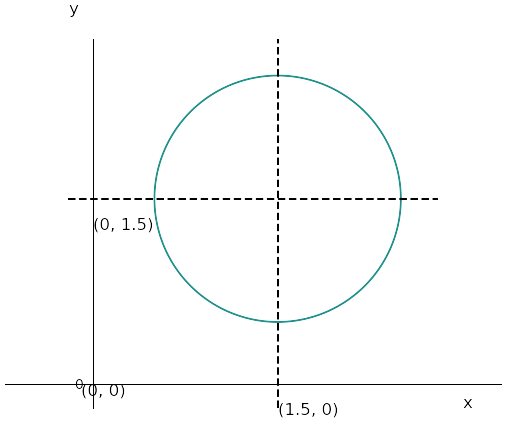
\includegraphics[width=0.45\columnwidth]{Img/jump1.png}\qquad
    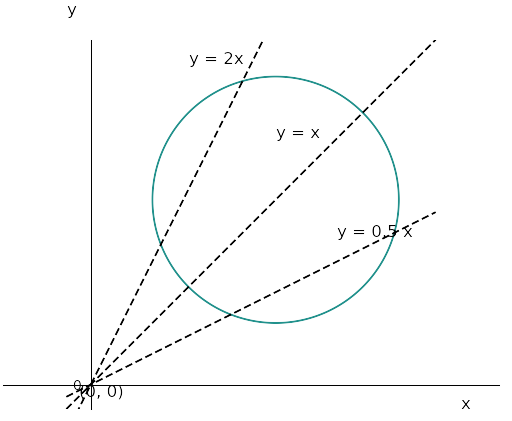
\includegraphics[width=0.45\columnwidth]{Img/jump2.png}
\label{fig:cell-jump}
\end{figure*}

\begin{example}
如图\ref{fig:cell-jump}所示,给定公式$F = \{(x - 1.5)^2 + (y - 1.5)^2 < 1\}$,赋值$\alpha_1 = \{x \mapsto 1.5, y \mapsto 0\}, \alpha_2 = \{x \mapsto 0, y \mapsto 1.5\}, \alpha_3 = \{x \mapsto 0, y \mapsto 0\}$。$F$在赋值$\alpha_1, \alpha_2, \alpha_3$下均不满足。

如\ref{fig:cell-jump}左图所示,当局部搜索算法选择初始赋值为$\alpha_1$时,通过平行y轴的胞腔跳跃可以得到操作$y \mapsto 1.5$使得不等式满足;同理当初始赋值为$\alpha_2$时,通过平行x轴的胞腔跳跃可以得到操作$x \mapsto 1.5$使得不等式满足。当局部搜索算法选择初始赋值为$\alpha_3$时,任何平行坐标轴的移动都不会使不等式满足,因此算法存在停滞的风险。

右图表示了基于固定直线的胞腔跳跃操作,定义三组方向向量分别为$dir_1 = \{1, 2\}, dir_2 = \{1, 1\}, dir_3 = \{2, 1\}$,对应的胞腔跳跃操作分别为$cjump(F, dir_1)$, $cjump(F, dir_2)$, $cjump(F, dir_3)$,替换后的多项式和可行域(保留三位小数)分别为:
\begin{align*}
    F_1 &= \{(t - 1.5)^2 + (2t - 1.5)^2 < 1\} \rightarrow (0.568, 1.232), \\
    F_2 &= \{(t - 1.5)^2 + (t - 1.5)^2 < 1\} \rightarrow (0.793, 2.207), \\
    F_3 &= \{(2t - 1.5)^2 + (t - 1.5)^2 < 1\} \rightarrow (0.568, 1.232).
\end{align*}
三个多项式的可行域均不为空,因此可以选取合适的值$t$同时移动变量$x$和$y$使得约束满足。
\end{example}

\section{基于变量级别可行域的操作缓存机制}
前述工作的胞腔跳跃操作都是基于单一子句进行的,通过收集所有不满足子句的操作最终决定最优的操作进行执行。但是,在实际的局部搜索迭代中,一个变量可能同时出现在多个子句中,因此在每次迭代中都需要重复计算变量的可行域。除此之外,基于单一子句的胞腔操作容易造成操作的冗余,从而减慢整体迭代效率。下面以例\ref{ex:jump}进行说明。

\begin{example}
\label{ex:jump}
考虑逻辑公式$F = \{P_1: (x-1)^2 + (y-1)^2 \leq 3, P_2: (x+1)^2 + (y-1)^2 \leq 3\}$,假设当前赋值为$\alpha: \{x \mapsto -1.5, y \mapsto 0.5\}$。可知当前赋值仅满足$P_1$,不满足$P_2$。考虑平行于x轴的胞腔跳跃操作$cjump(P_1, x)$,即图\ref{fig:jump2}中虚线所示。

\begin{figure*}[t]
    \centering
    \bicaption {基于变量级别可行域的胞腔跳跃操作} {Cell-jump operation based on variable-level feasible-set}
    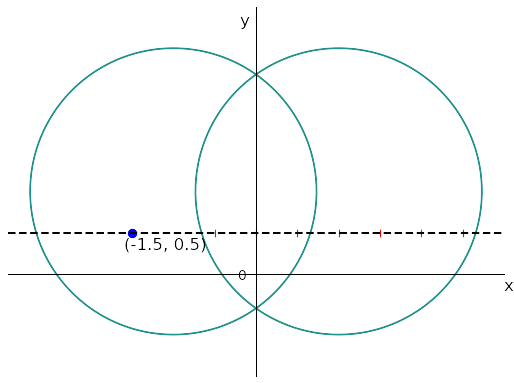
\includegraphics[width=0.45\columnwidth]{Img/op1.png}\qquad
    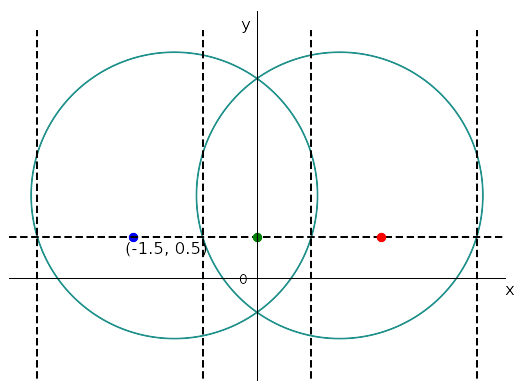
\includegraphics[width=0.45\columnwidth]{Img/op2.png}
\label{fig:jump2}
\end{figure*}

\textbf{传统计算方法(图\ref{fig:jump2}左图):}
\begin{itemize}
    \item 首先计算变量$x$对约束$P_1$的可行域$(-0.658, 2.658)$。
    \item 根据可行域进行采样,比如选取7个采样点得到$\{-0.5, 0, 0.5, 1, 1.5, 2, 2.5\}$,如图\ref{fig:jump2}左图中短竖线所示。
    \item 对这5个采样点逐一计算分数,选取其中分数最大的操作,比如$\{x \mapsto 0\}$。
    \item 移动后的赋值$\{x \mapsto 0, y \mapsto 0.5\}$满足约束$P_1$和$P_2$,找到可行解,算法停止。
\end{itemize}

这种方法带来了两个潜在的问题:
\begin{enumerate}
    \item 因为目前的胞腔跳跃操作$cjump(P_1, x)$是基于单一约束设计的,因此选择的采样点有可能同时破坏当前已经满足的约束。虽然可以通过打分函数进行筛选,但更好的方式是选择操作的时候进行简单判断。图\ref{fig:jump2}左图中,红色采样点表示破坏了原先$P_2$的可满足状态,而绿色采样点表示保持了$P_2$的可满足状态。
    \item 在每次迭代中,本工作只会根据当前约束的可行域进行采样,因此可能造成整体$R^n$空间上同类操作的冗余,从而在接下来的打分函数计算环节降低了算法的效率。比如在图\ref{fig:jump2}左图中,红色竖线同属一个胞腔,绿色竖线同属另一个胞腔,同一个胞腔对SMT公式的影响完全相同,没必要重复计算。
\end{enumerate}

\begin{definition}{\textbf{同类操作(Similar Operations)}}
    对于多项式约束$P$,给定两个胞腔跳跃操作$cjump_1(P, x)$和$cjump_2(P, x)$,他们分别将变量$x$移动到不同的赋值。如果两个移动后的赋值$\alpha_1$和$\alpha_2$在解空间上存在于同一个胞腔中,定义两个操作是同类操作,记作$cjump_1(P, x) \sim cjump_2(P, x)$。
\end{definition}
从图中可以看出,更好地刻画胞腔跳跃操作需要引入变量在多个子句的可行域概念,综合所有可行域后才能可以得到可行域-分数的对应关系。改进的计算方法描述如下:

\textbf{改进计算方法(图\ref{fig:jump2}右图):}
\begin{itemize}
    \item 首先计算变量$x$对两个约束$P_1$和$P_2$各自的可行域: $(-0.658, 2.658)$和$(-2.658, 0.658)$。
    \item 综合两个可行域,可以得到$R$上的一个划分:$(-2.658, -0.658)$, $(-0.658, 0.658)$, $(0.658, 2.658)$。
    \item 对于每一个部分,只需要选择一个采样点即可,然后计算当前操作的得分,选择分数最佳的操作。如图\ref{fig:jump2}右图中,选择了红色$(0, 0.5)$和绿色$(1.5, 0.5)$两个采样点,前者同时满足两个约束,而后者仅仅满足$P_1$约束。
    \item 检查移动后的赋值$\alpha: \{x \mapsto 0, y \mapsto 0.5\}$,找到可行解,算法停止。
\end{itemize}
比较两种算法,可以看出传统算法采样在单一子句可行域计算时进行,也仅仅维护了赋值-分数的对应关系;而改进后的算法通过综合多个子句的可行域,维护了$R$上每一个赋值和分数的映射关系,可以非常方便计算出对应的操作分数。除此之外,因为传统算法提前采样的特点,产生了大量的冗余操作,改进后的算法因为直接在胞腔层面进行了维护,因此采样点的选择更具有合理性。
\end{example}

本文把$R$上胞腔的分割定义为\textbf{边界(boundary)},具体定义如下:
\begin{definition}{\textbf{边界(boundary)}}
本文定义\textbf{边界(boundary)}为一种四元组数据结构$<val, is\_open, is\_make, cid>$,其中$val$是实数,表示边界的值,$is\_open$是布尔值,表示边界是否为开区间,$is\_make$是布尔值,表示边界处分数递增还是递减,$cid$表示该处边界对应的子句编号。定义边界之间的排序为:首先$val$值小的排在前面,如果$val$相同,$is\_open$为假的排在前面,这样可以得到一组按照实数自然排序的边界集合(boundary set)。
\end{definition}
需要注意的是,边界仅仅刻画变量从边界左侧移动到边界右侧对应的约束变化情况(可满足到不可满足,不可满足到可满足),如果要计算对应胞腔的具体分数,需要从边界处采样点进行计算。下面使用例\ref{ex:jump2}进行说明。

\begin{example}
\label{ex:jump2}
\begin{figure*}[t]
    \centering
    \bicaption {边界计算示意图} {Demo of Coomputation of Boundaries}
    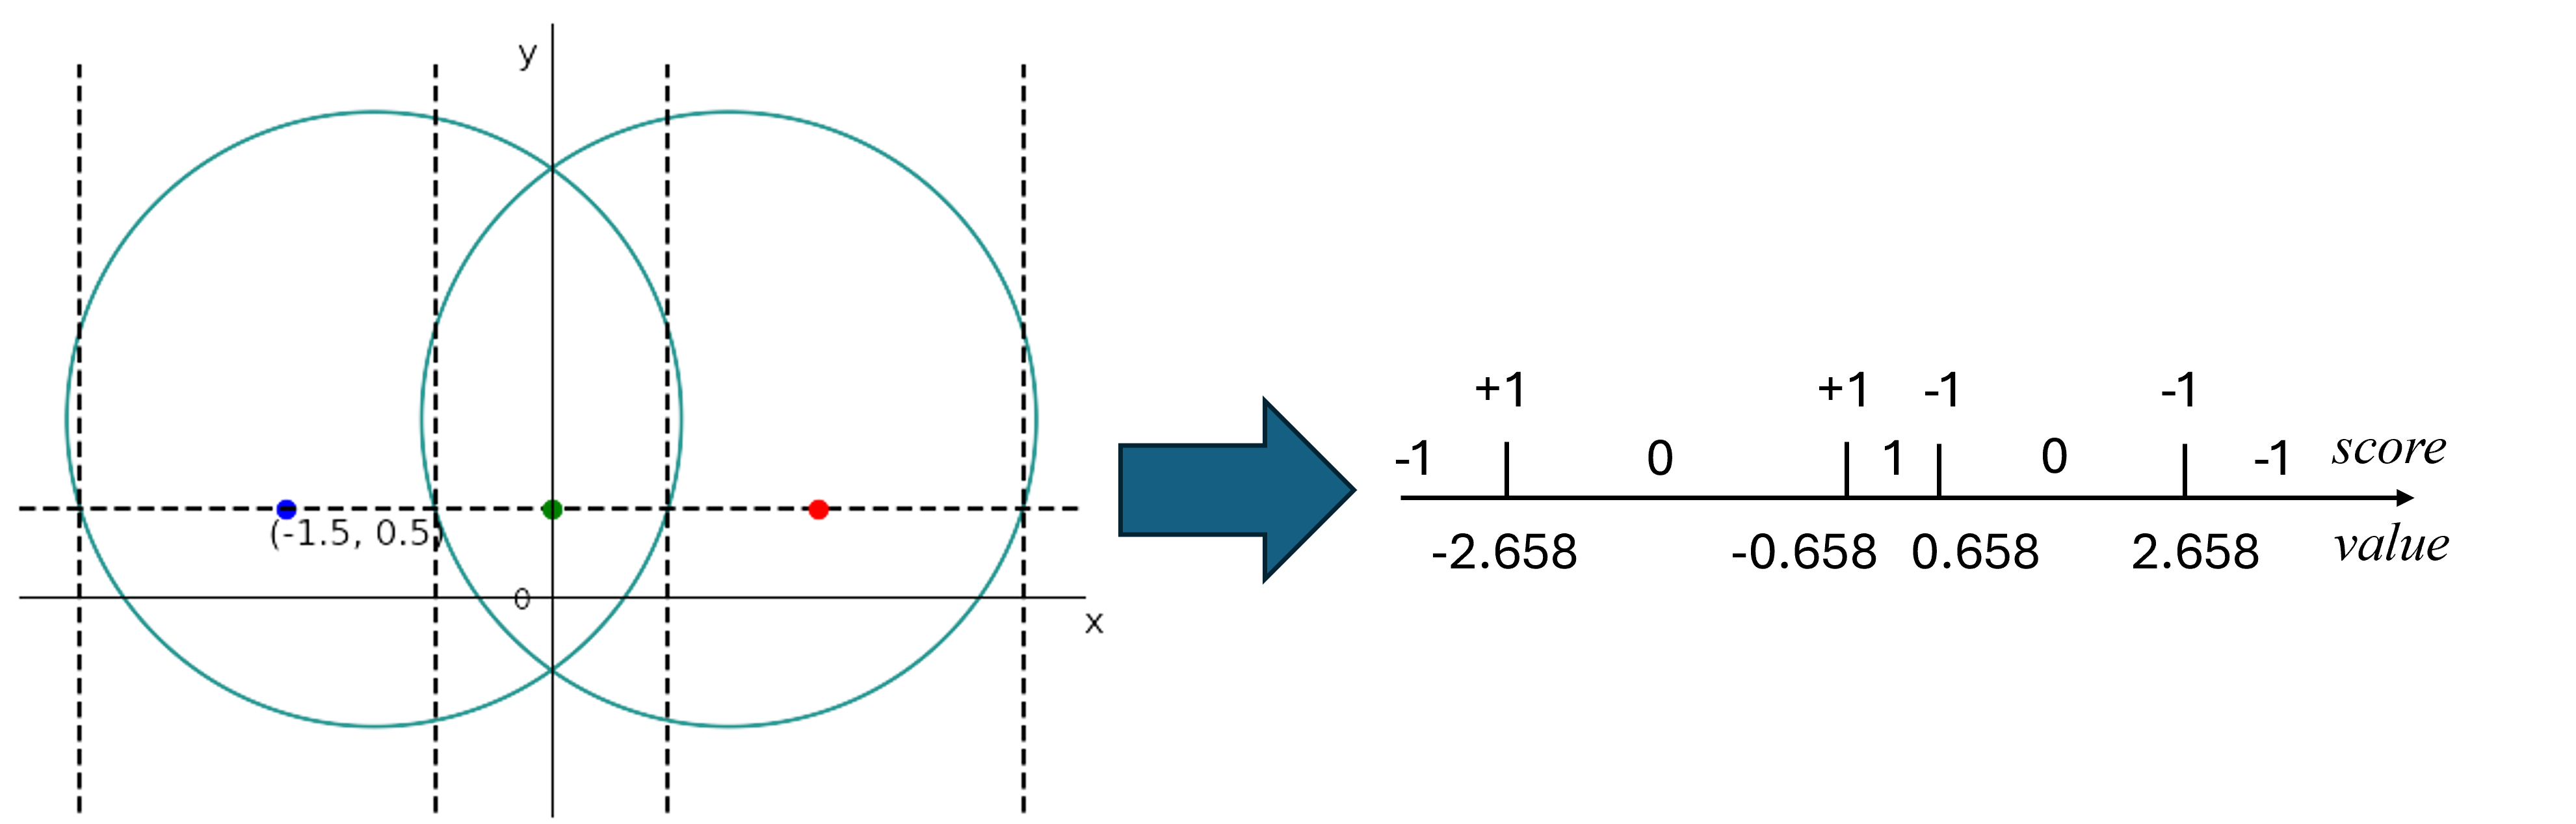
\includegraphics[width=\columnwidth]{Img/boundary.png}
\label{fig:boundary}
\end{figure*}

仍然考虑例\ref{ex:jump}中的约束和赋值,约束$P_1$和$P_2$的可行域是:$(-0.658, 2.658)$和$(-2.658, 0.658)$。在边界处,变量从左向右移动会导致相应约束的满足状态发生变化,假设每个约束的权重为1,可以计算得到$R$上的四个边界如下:
\begin{align}
Boundary_1 &: <-2.658, \top, \top, 2> \nonumber \\
Boundary_2 &: <-0.658, \top, \top, 1> \nonumber \\
Boundary_3 &: <0.658, \bot, \bot, 1> \nonumber \\
Boundary_4 &: <2.658, \bot, \bot, 2> \nonumber
\end{align}
四次边界处的分数变化均为1。为了求得赋值和分数的对应关系,需要在每个分割的胞腔处采样,然后计算分数。一种更简单的办法是计算某一个胞腔处的分数,然后根据边界的分数变化计算其他胞腔处的分数。可以注意到,当变量$x$移动到和原来赋值所在的胞腔时(比如例子中的$(-2.658, -0.658)$),对应的分数一定为0。为了计算的方便性,本文引入\textbf{起始分数(starting score)}的概念来表示数轴最左侧代表的分数。

\begin{definition}{\textbf{起始分数(Starting Score)}}
本文定义起始分数为一个实数值,表示数轴上最左侧点对应的分数,即变量移动到$-\infty$时对应的分数。
\end{definition}
在本例子中,最左侧的赋值会破坏原先已经满足的$P_2$约束,因此分数为-1。在每次边界处增加或减少对应的分数,因此可以得到图\ref{fig:boundary}右侧的结果。边界和分数的计算展示在算法\ref{alg:score}中。
\end{example}

\begin{algorithm}[t]
    % \small
    \caption{Computation of best critical move and score}
    \label{alg:score}
    \textbf{输入}: variable $x$, boundary set $B$ and starting score $s_0$\\
    \textbf{输出}: Best critical move range $val$ and score $score$
    \begin{algorithmic}[1] %[1] enables line numbers
        \Statex \hrulefill

        \State $score \leftarrow -\infty$;
        \State $s \leftarrow s_0$;
        \FOR{each boundary $b$ in $B$}
            \STATE $s \leftarrow s + s_{change}$;
            \IF{$s > score$}
                \STATE $score \leftarrow s$;
                \STATE $val \leftarrow b.val$;
            \ENDIF
        \ENDFOR
        \RETURN $val$ and $score$
    \end{algorithmic}
\end{algorithm}

在局部搜索算法中,每一次迭代只会改变一个变量的赋值,因此绝大多数约束的可满足状态和可行域不会发生变化,一个可行的优化是增量式计算变量的边界集合。具体而言,当一个变量的赋值发生改变时,只有其所在的约束会发生相应的赋值变化,只有那些约束所包含的变量的边界需要更新。为方便说明,本文定义邻居变量的概念如下:

\begin{definition}{\textbf{邻居变量(Neighbor Variables)}}
    对于变量$x$,其所在的约束集合记为$C_x$,那么$x$的邻居变量集合$N_x$定义为$N_x = \{y | \exists c \in C_x, y \in Var(c) \land y \neq x\}$。
\end{definition}

\begin{algorithm}[t]
    % \small
    \caption{Incremental computation of make-break move and scores}
    \label{alg:update}
    \textbf{输入}: Variable $v$ that is modified\\
    \textbf{更新}: Make-break move and scores
    \begin{algorithmic}[1] %[1] enables line numbers
        \Statex \hrulefill

        \State $V \leftarrow \emptyset$;
        \FOR{each clause $cls$ that contains $v$}
            \FOR{variable $v'$ in $cls$}
                \STATE $V \leftarrow V \cup \{v\}'$;
                \STATE boundary $bd \leftarrow $ compute boundary of $v'$ with respect to  $cls$;
                \STATE add $bd$ to boundary set $S_{v'}$;   
            \ENDFOR
        \ENDFOR

        \FOR{variable $v'$ in $V$}
            \STATE recompute best critical move and score for $v'$; \Comment{algorithm \ref{alg:score}}
        \ENDFOR
    \end{algorithmic}
\end{algorithm}

在具体实现中,本算法为每一个变量维护一个边界集合$S_vx$,当一次迭代带来变量$v$赋值发生变化后,重新计算其包含的每个约束$c$对邻居变量$v'$的新边界,然后更新到其边界集合$S_{v'}$中。在所有边界更新完毕后,对每个邻居变量$v'$重新计算其最佳的边界和分数,以方便下一次算法迭代。算法\ref{alg:update}展示了伪代码。

下面的例子\ref{ex:update}展示了边界计算的更新过程。

\begin{example}
\label{ex:update}
考虑约束集合$F = \{P_1: x^2 + y^2 \leq 1, P_2: x + y < 1, P_3: x + z > 0\}$。当前赋值为$\alpha: \{x \mapsto 1, y \mapsto 1, z \mapsto 1\}$,所有约束权重为1。则当前状态每个约束关于变量$x$的可行域和边界计算如下:
\begin{align}
& x^2 + y^2 \leq 1  \rightarrow x \in [0, 0] \nonumber & \quad \text{Boundary: } & \{<0, \bot, \top, 1>, <0, \top, \bot, 1>\} \nonumber \\
& x + y < 1  \rightarrow x \in (-\infty, 0) \nonumber & \quad \text{Boundary: } & \{<0, \bot, \bot, 1>\} \nonumber \\
& x + z > 1  \rightarrow x \in (-1, +\infty) \nonumber & \quad \text{Boundary: } & \{<-1, \top, \top, 1>\} \nonumber
\end{align}
排序后的边界集合为:
$$
\{<-1, \top, \top, 1>, , <0, \bot, \top, 1>, <0, \top, \bot, 1>, <0, \bot, \bot, 1>\}
$$

当某次迭代发生赋值$y \mapsto -2$时,约束$x + y < 1$有不满足状态变为可满足状态。由于变量$y$和$z$不为邻居变量(没有共同存在的约束),因此无需更改变量$z$的边界。对于前两个同时存在变量$x$和$y$的子句,需要重新计算关于变量$x$的边界信息。

\begin{align}
& x^2 + y^2 \leq 1  \rightarrow x \in \emptyset \nonumber & \quad \text{Boundary: } & \emptyset \nonumber \\
& x + y < 1  \rightarrow x \in (-\infty, 3) \nonumber & \quad \text{Boundary: } & \{<3, \bot, \bot, 1>\} \nonumber
\end{align}
排序后的边界集合为:
$$
\{<-1, \top, \top, 1>, <3, \bot, \bot, 1>\}
$$
\end{example}

除了本章节提到的设计之外,边界信息的维护仍然存在以下几种优化空间:
\begin{itemize}
    \item \textbf{更复杂的数据结构:}除了使用边界(线性数据结构)维护变量赋值-分数关系之外,也可以使用二叉树等顺序存储的数据结构。一般来说,当变量的边界个数很小时(SMT-LIB中大多数样例),现行的数据结构已经足够高效。对于更多操作,二叉搜索树也许更为高效。
    \item \textbf{迭代优化:}在每次迭代中,由于本算法只会从未满足子句中选择操作,因此可以只更新那些出现在未满足子句中的变量的边界信息,而不是所有的邻居变量。除此之外,可以使用更懒惰的办法,比如为特定需要更新的约束打标记,然后在其不可满足时才更新边界信息。
\end{itemize}

\section{本章小结}
本章节首先回顾了以往工作提出的用于求解算术SMT问题的胞腔跳跃操作,具体包括平行坐标轴和沿固定直线两种方法。然后,本文根据一个例子指出了以往针对单个子句的胞腔操作存在冗余问题,并且在迭代过程中容易造成可行域缓存的损失,基于此本文给出了边界和同类操作的定义以及操作缓存机制。最后,本工作给出了邻居变量的定义,并借此给出可行域缓存机制的迭代条件,即只有邻居变量的赋值发生变化时才需要更新边界信息。本工作还讨论了可能的优化,比如更复杂的数据结构或者更新条件等。